\chapter{System Setup} \label{ch:system-setup}

The Shadow Dexterous Hand~\cite{shadow-dex-hand} is a sophisticated robotic hand with \num{24} \gls{dof} and a wide range of sensory feedback capabilities. To develop and test control algorithms for this complex system, simulation is an invaluable tool. In this chapter, the practical setup of our project is presented, which involves simulating the Shadow Dexterous Hand in Gazebo~\cite{gazebo} within a Docker container~\cite{docker}. \medskip

This simulation is based on the Shadow Robot Company's~\cite{shadow-robotics} \gls{ros}~\cite{ros} packages~\cite{shadow-ros-packages}, which provide a flexible and customizable framework for controlling the hand. This project uses Gazebo, a popular robot simulation environment, to simulate the physics of the hand and its interaction with the environment. To ensure reproducibility and portability, the development framework which encapsulates the simulation environment is built within a Docker container, which allows us to easily distribute our code and dependencies to other researchers. \medskip

In this chapter, a detailed description of the hardware and software used in this project's simulation setup is provided, which includes the software architecture of the simulation, including the ROS packages and Gazebo plugins used to simulate the hand and its environment.

% Additionally, we detail the data collection and processing methods used in our simulation, including the types of data collected and how it is processed. We provide a code snippet to illustrate the structure and functionality of our simulation, and we include relevant diagrams and figures to help clarify the technical information.

% By simulating the Shadow Dexterous Hand in Gazebo within a Docker container, we can develop and test control algorithms in a safe, efficient, and easily reproducible manner. This chapter provides a comprehensive overview of our simulation setup and serves as a foundation for the subsequent chapters that detail our experimental results and analysis.

\section{Simulation Setup} \label{sec:system-setup-simulation-setup}

The \gls{cad} model of the Shadow Dexterous Hand is a highly detailed and accurate representation of the physical hand. The model is based on the original design of the real-world hand, which was developed by the Shadow Robot Company. \medskip

The \gls{cad} model includes precise geometry for all of the hand's components, including the finger joints, tendons, and tactile sensors. The model also includes detailed material properties for each component, which are used to simulate the hand's physical behavior in the simulation.\medskip

The structure of the hand can be seen in \figref{fig:robot-hand-skeleton} compared to a human hand in \figref{fig:human-hand-skeleton}

\begin{figure}[h]
	\centering
	\begin{subfigure}[b]{0.48\textwidth}
		\centering
		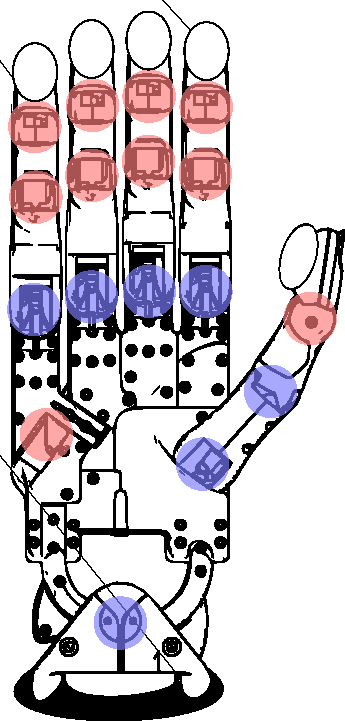
\includegraphics[height=\textwidth]{chapters/system-setup/fig/robot-hand-skeleton.pdf}
		\caption{Shadow Dexterous hand with joints color coded depending on the degrees of freedom. The total number of degrees of freedom can here be seen as \num{24}.}
		\label{fig:robot-hand-skeleton}
	\end{subfigure}
	\hfill
	\begin{subfigure}[b]{0.48\textwidth}
		\centering
		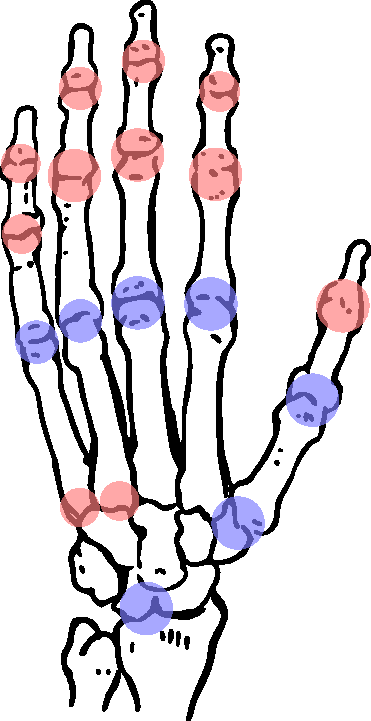
\includegraphics[height=\textwidth]{chapters/system-setup/fig/human-skeleton-hand.pdf}
		\caption{Shadow Dexterous hand with joints color coded depending on the degrees of freedom. The total number of degrees of freedom can here be seen as \num{25}~\cite{design-and-development-of-a-bilateral-therapeutic-hand-device-for-stroke-rehabilitation}.}
		\label{fig:human-hand-skeleton}
	\end{subfigure}
	\caption{The Shadow Dexterous hand and a human hand red here marks a joint with \num{1} degree of freedom, while blue marks a joint with \num{2}.}
	\label{fig:hands-dof}
\end{figure}

The hand's geometry is modeled using a combination of standard shapes and custom-designed components. For example, the finger joints are modeled using a series of cylinders and spheres, which are connected by virtual tendons to simulate the motion of the real-world hand. The tactile sensors are modeled as a grid of small, deformable elements, which provide a high-resolution map of the contact forces between the hand and its environment.\medskip

While the model does not support representative tactile sensors in Gazebo at the writing of this project.


To ensure that the \gls{cad} model accurately reflects the behavior of the real-world hand, we have incorporated data from physical experiments into our simulation. For example, we have used force sensors to measure the forces and torques applied to the hand during grasping and manipulation tasks. We have also used high-speed cameras to capture the hand's motion and behavior in different scenarios.\medskip


The simulated hand structure


added tactile sensor extension



\section{Software Setup} \label{sec:system-setup-software-setup}



